\documentclass[titlepage]{scrartcl}
\usepackage{enumitem}
\usepackage[british]{babel}
\usepackage[style=apa, backend=biber]{biblatex}
\DeclareLanguageMapping{british}{british-apa}
\usepackage{url}
\usepackage{float}
\usepackage[labelformat=empty]{caption}
\restylefloat{table}
\usepackage{perpage}
\MakePerPage{footnote}
\usepackage{abstract}
\usepackage{graphicx}
% Create hyperlinks in bibliography
\usepackage{hyperref}
\usepackage{amsmath}

\usepackage[T1]{fontenc}
\usepackage[utf8]{inputenc}
\usepackage{blindtext}
\setkomafont{disposition}{\normalfont\bfseries}

\graphicspath{
    {./resources/},
}
\addbibresource{ ~/Documents/library.bib }

\newsavebox{\abstractbox}
\renewenvironment{abstract}
  {\begin{lrbox}{0}\begin{minipage}{\textwidth}
   \begin{center}\normalfont\sectfont\abstractname\end{center}\quotation}
  {\endquotation\end{minipage}\end{lrbox}%
   \global\setbox\abstractbox=\box0 }

\usepackage{etoolbox}
\makeatletter
\expandafter\patchcmd\csname\string\maketitle\endcsname
  {\vskip\z@\@plus3fill}
  {\vskip\z@\@plus2fill\box\abstractbox\vskip\z@\@plus1fill}
  {}{}
\makeatother

\DeclareCiteCommand{\citeyearpar}
    {}
    {\mkbibparens{\bibhyperref{\printdate}}}
    {\multicitedelim}
    {}

% MATLAB Code block stuff...
\usepackage{color}
\usepackage{listings}

\definecolor{dkgreen}{rgb}{0,0.6,0}
\definecolor{gray}{rgb}{0.5,0.5,0.5}

\lstset{language=Matlab,
    keywords={break,case,catch,continue,else,elseif,end,for,function,
        global,if,otherwise,persistent,return,switch,try,while},
    basicstyle=\ttfamily,
    keywordstyle=\color{blue},
    commentstyle=\color{gray},
    stringstyle=\color{dkgreen},
    numbers=left,
    numberstyle=\tiny\color{gray},
    stepnumber=1,
    numbersep=10pt,
    backgroundcolor=\color{white},
    tabsize=4,
    showspaces=false,
    showstringspaces=false
    frame=single,
    breaklines=true,
    %postbreak=\raisebox{0ex}[0ex][0ex]{\ensuremath{\color{red}\hookrightarrow\space}}
}

\begin{document}
\title{ECS707P - DSP}
\subtitle{\LARGE{Lab 3}}
\author{Sam Perry - ec16039}

\maketitle

\section{Using 32 samples of a sinusoid with frequency 220 Hz, sampled at a
constant rate of 2,048 Hz, zeropad it to a total length of 1024 samples and
calculate the DFT of the result. Plot this using a line, and overlay this with
a stem plot of the DFT of the original 32 samples.}
\begin{lstlisting}
% Main function for running exercises
function main()
    % Declare the number of samples in the sine wave
    N = 32;
    % Declare the sample rate
    fs = 2048;
    % Create indexes 1 - N time = [0:N-1];
    % Declare the frequency as 220Hz
    frequency = 220;
    % Declare the amplitude
    amplitude = 1.0;

    % Generate signal x from parameters
    x = amplitude * sin(2*pi*frequency*(time/fs));

    % Compute the DFT of the sine wave
    X = fft(x);
    
    % Pad with zeros to make vector 2048 samples long
    X2 = fft([x, zeros(1, 2048-N)]);


    % Calculate absolute magnitude of spectrum
    X = abs(X);
    X2 = abs(X2);

    % Zero pad smaller vector so they are the same sie for plotting
    % Kronecker padding technique taken from: http://stackoverflow.com/questions/11776251/inserting-variable-number-of-zeros-between-non-zero-elements-in-a-vector-in-matl
    zero_p = length(X2) / length(X)
    b = [1 zeros(1,zero_p-1)];
    X = kron(X, b)
    X(X == 0) = NaN

    figure

    % Plot the absolute magnitude of the DFT to a graph
    stem(X(1:2048/2));
    hold on
    plot(X2(1:2048/2));
    % Set xlabel to show bin 10 bin indexes
    set(gca,'XTickMode','manual');
    set(gca,'XTick',int64((1:10)*(1024/10)));
    set(gca,'XtickLabels',int64((1:10)*((fs/2)/10)));


    % Turn on grid
    grid on;
    
    % Add a title to the graph
    title('DFT of x')
    
    % Label the x axis as 'Frequency'
    xlabel('Bin Index')
    % Label the y axis as 'Magnitude'
    ylabel('Magnitude |X|')
\end{lstlisting}

\begin{figure}[H]
    \caption{32 point DFT (blue) and 2048 point zero padded DFT (red) of a
    32 sample 220Hz Sine Wave}
    \makebox[\textwidth]{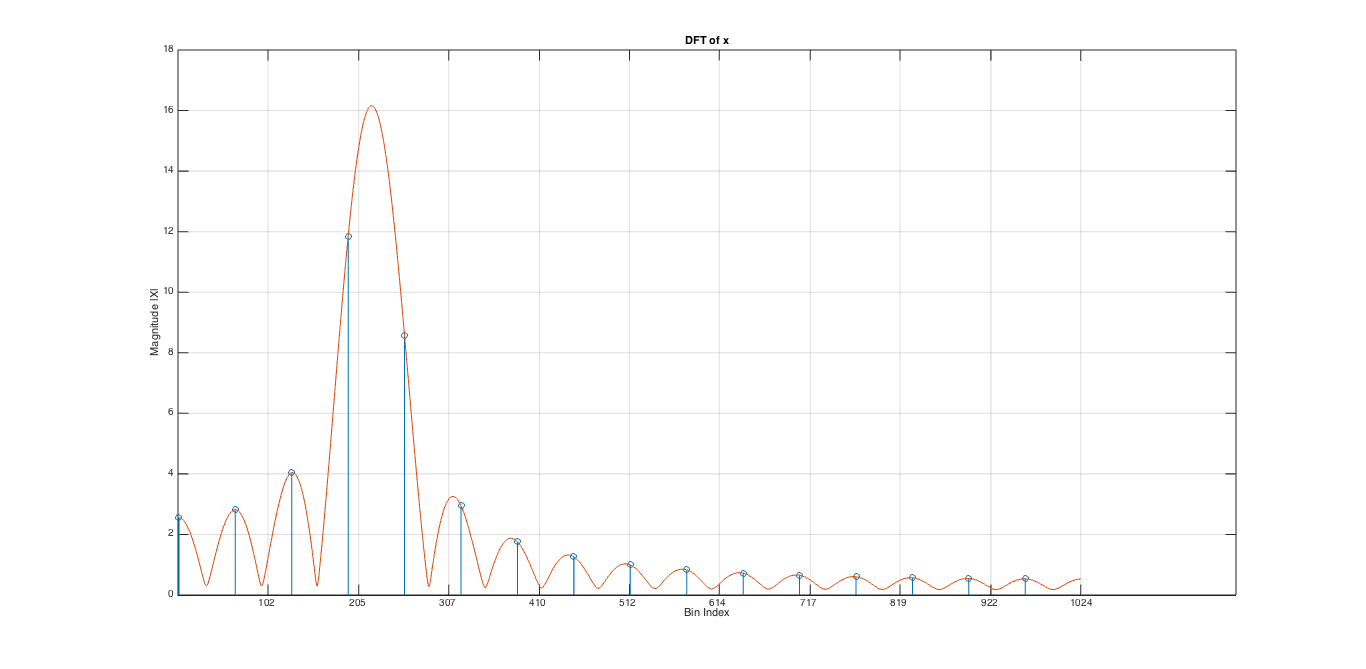
\includegraphics[width=1.1\textwidth]{ZeropadDFT1}}
    \label{ZeropadDFT1}
\end{figure}

\section{Using your code from 1.1, reduce the frequency of the sinusoid to 128
Hz and run it again. Include just the plot and comment on what has happened.}
\begin{figure}[H]
    \caption{32 point DFT (blue) and 2048 point zero padded DFT (red) of a 32
    sample 128Hz sine wave}
    \makebox[\textwidth]{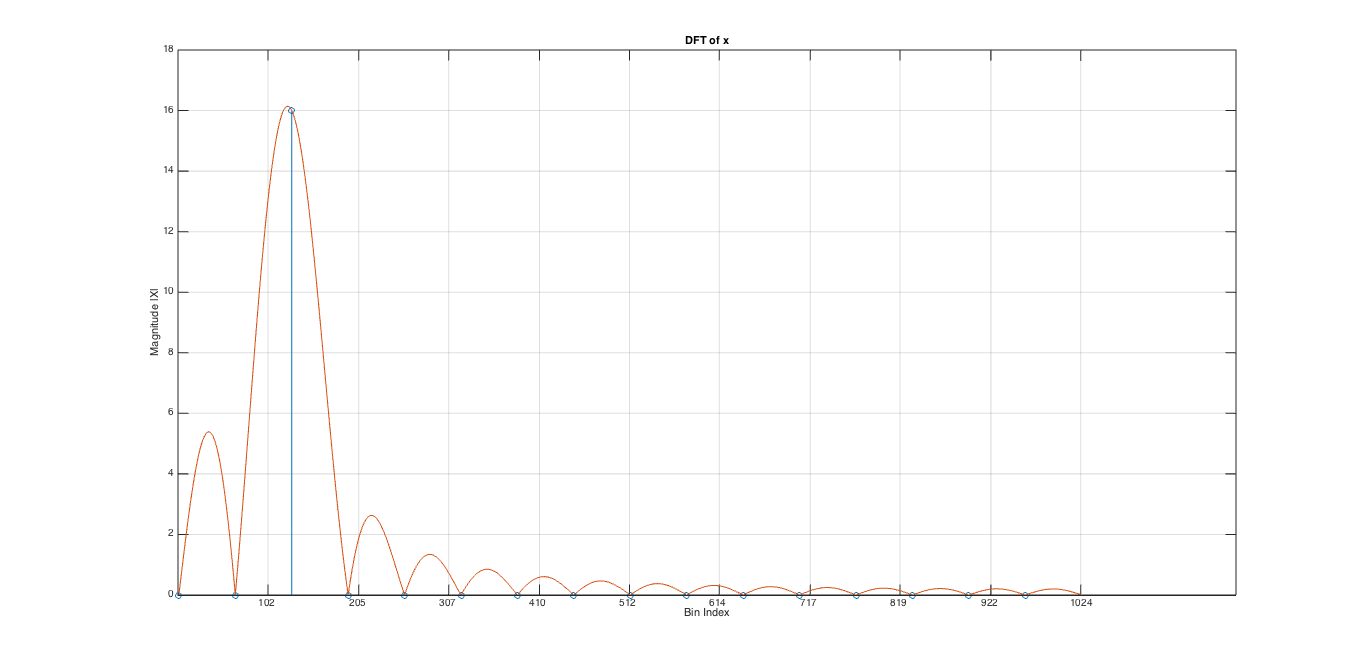
\includegraphics[width=1.1\textwidth]{ZeropadDFT2}}
    \label{ZeropadDFT2}
\end{figure}

The extra lobes that can be seen in the 2048 point DFT are a result of the
zeropadding applied to the signal. By adding zeros to the signal, a rectangular
window is effectively applied to the signal, causing a discontinuity in the
signal. This produces the lobes that appear in the 2048 point DFT shown.
\pagebreak
\section{Using the same code in 1.1, perform a DFT of a length-32 signal that
    is a sum of the following three
    sinusoids:
    $$x[n]=sin(2\pi128n\div2048)+0.2sin(2\pi220n\div2048)+0.01cos(2\pi525n\div2048)$$
    Also find the DFT of the signal zeropadded to a length 2048. Overlay
    the
DFT spectrum of length-32 using stem, with the zero-padded DFT
    spectrum
€
using plot, an example of which is seen in Figure 5. Include
just your plot.}
\begin{figure}[H]
    \caption{32 point DFT (blue) and 2048 point zero padded DFT (red) of a 32
    sample 3 partial sine wave}
    \makebox[\textwidth]{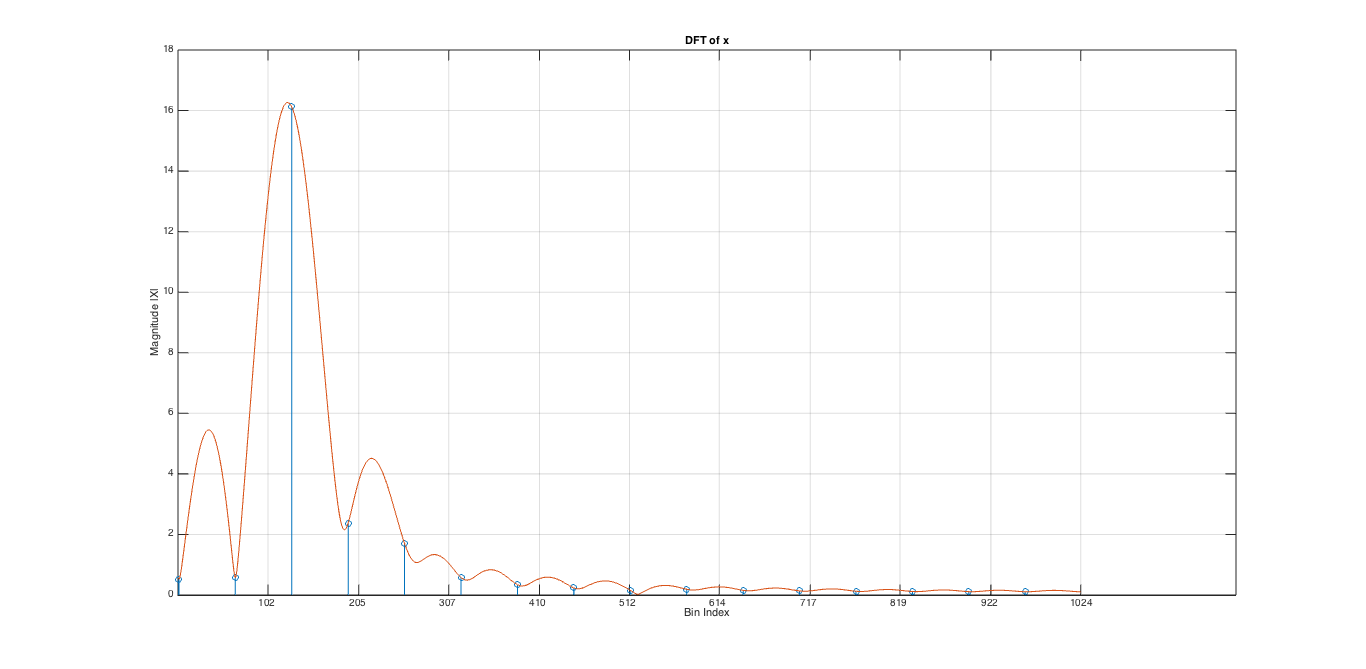
\includegraphics[width=1.1\textwidth]{ZeropadDFT3}}
    \label{ZeropadDFT3}
\end{figure}

\section{Without the knowledge that there are multiple pure tones in this
sequence, can you pick out the right frequency components in the magnitude
spectrum?}
The 128Hz sine wave can be seen as the largest peak in the magnitude spectrum.
However, the other tones are much harder to distinguish. Their lobes are merged
into the lobes of the other tones and as their amplitude is not significantly
high, they become unrecongisable as tones.

\section{Program the four windows above. Using N=31 for the triangular
window, and N=32 for the others, plot each window on the same graph (using plot
instead of stem) and label each using gtext}

\begin{figure}[H]
    \caption{Rectangle (cyan, $N=32$), Hann (red, $N=32$), Sine (green, $N=32$) and Triangular (blue, $N=31$)
    windows }
    \makebox[\textwidth]{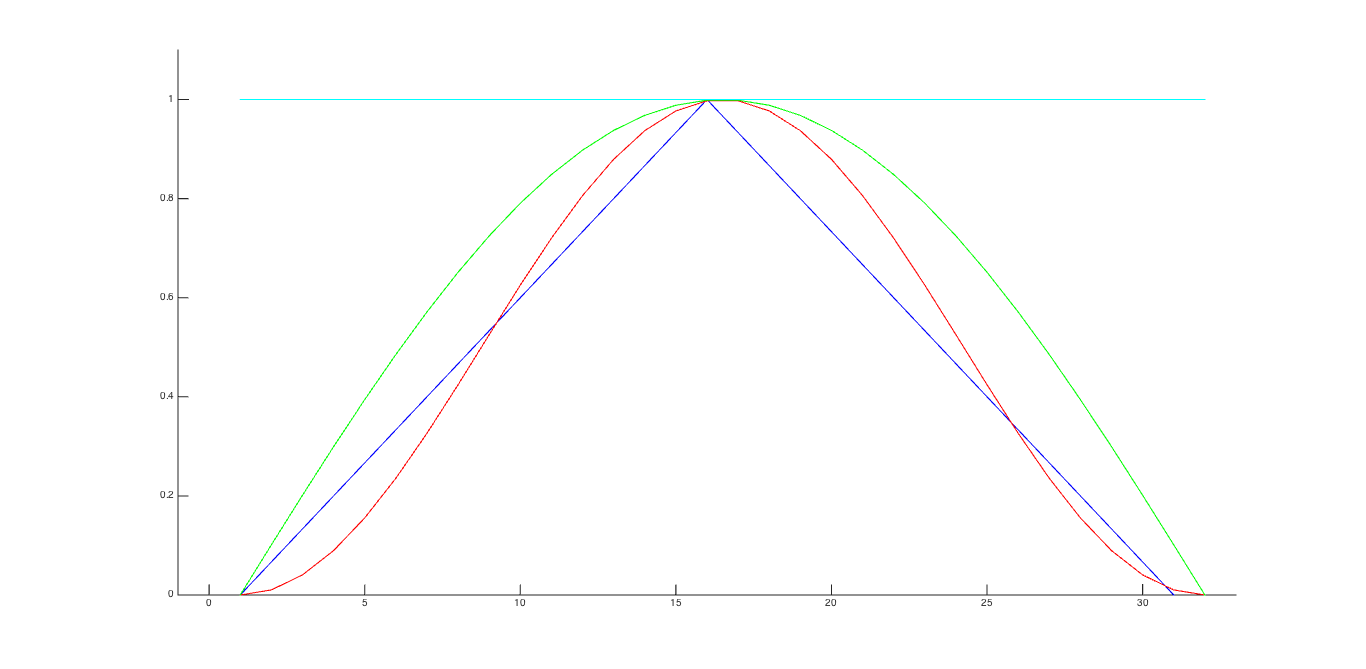
\includegraphics[width=1.1\textwidth]{windows}}
    \label{windows}
\end{figure}

\section{Plot the normalized magnitude spectrum (not dB) as a function of
normalized frequency of each window on four different plots}
\begin{figure}[H]
    \caption{1024 point DFT of 32 point Triangle, Rectangle, Sine and Hann
    windows}
    \makebox[\textwidth]{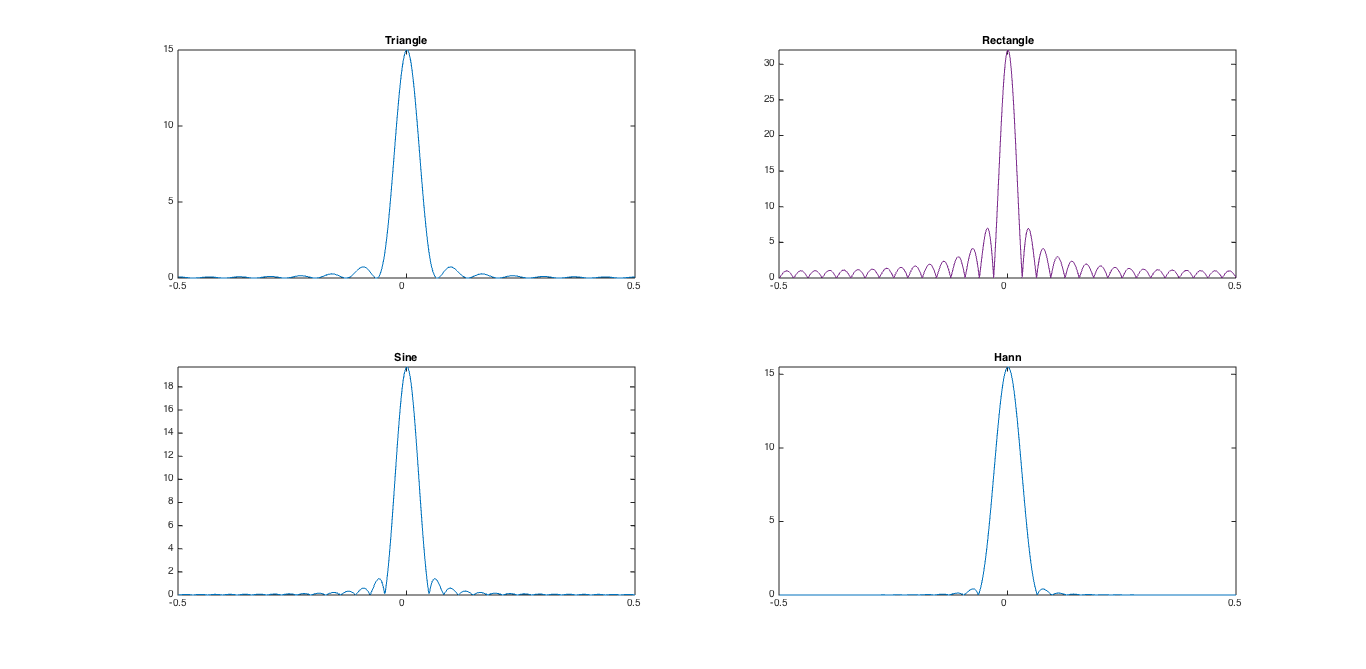
\includegraphics[width=1.1\textwidth]{4WinFFT}}
    \label{4WinFFT}
\end{figure}

\section{For the spectra found in 2.2, plot the normalized dB spectrum of the
rectangular and triangular window functions (1-2), on the same graph}
\begin{figure}[H]
    \caption{Peak Magnitude Lobes of Triangle and Rectangle Windows}
    \makebox[\textwidth]{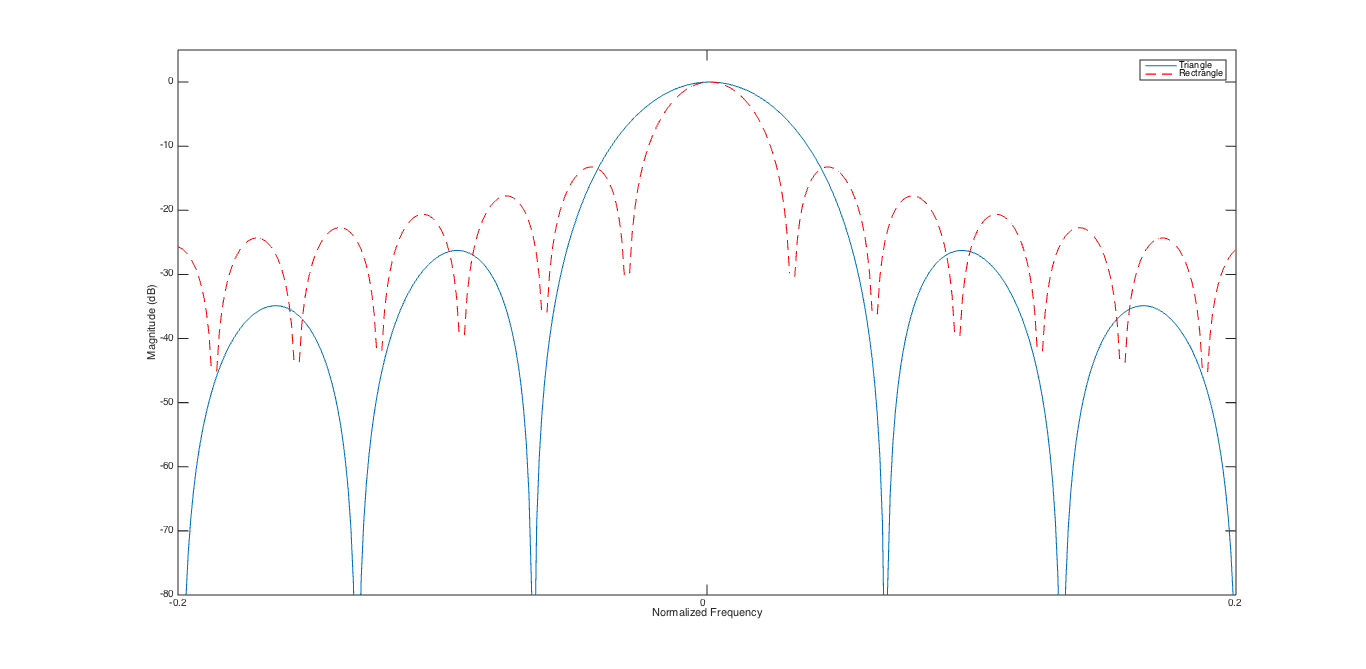
\includegraphics[width=1.1\textwidth]{TriRectDFT}}
    \label{TriRectDFT}
\end{figure}

\section{Find the width of the main-lobe for these two windows. What is the
width of the main-lobe for the triangular window in terms of that for the
rectangular window? Do you have any intuition why this is the case?} The width
of the rectangular window is half that of the triangular window. The triangular
window weights samples by linearly decrasing values symetrically around the
signal's center, resulting in an increased reduction in side lobe magnitude as
distance increases from the main lobe. This comes at the cost of an increased
(doubled) main lobe size. 

\section{At what magnitude dB is the height of the first side-lobe for the
rectangular and triangular windows?}
The magnitude peaks at -26.26 for the triangular window. It peaks at -13.23 for
the rectangular window.

\section{Repeat 2.3 for the Sine and Hann window functions (3-4)}
\begin{figure}[H]
    \caption{Peak Magnitude Lobes of Sine and Hann Windows}
    \makebox[\textwidth]{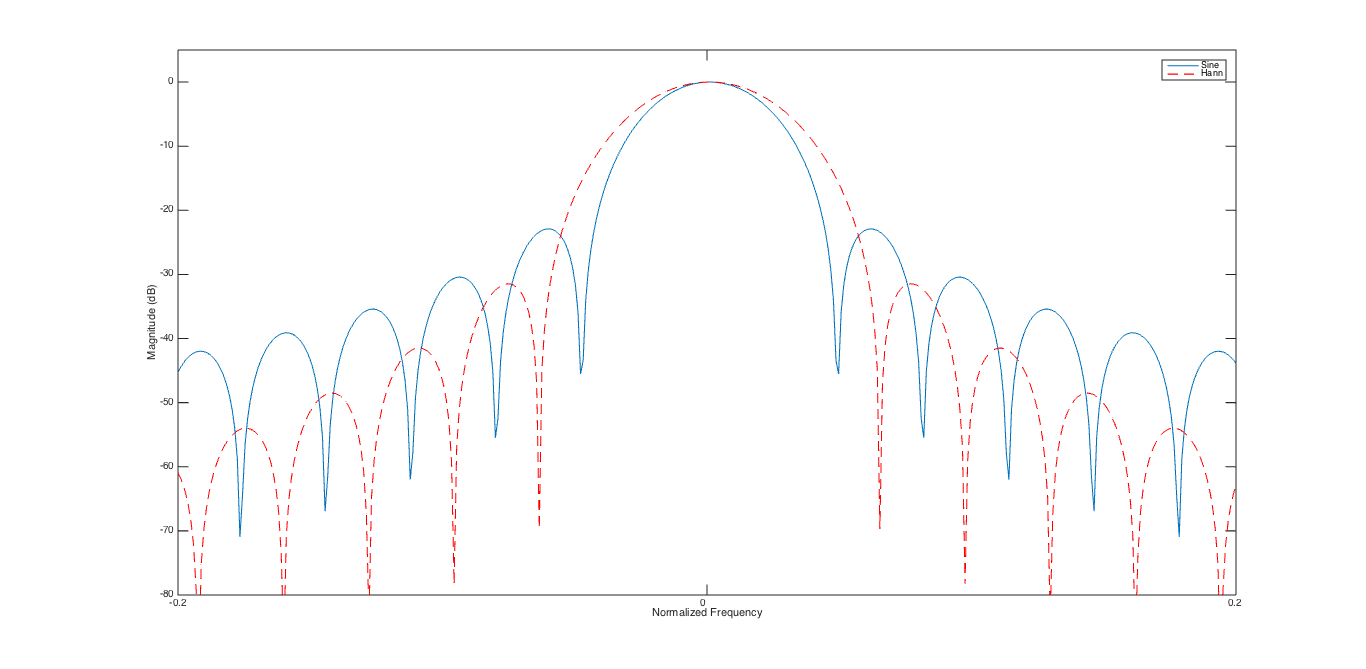
\includegraphics[width=1.1\textwidth]{SineHannDFT}}
    \label{SineHannDFT}
\end{figure}

\section{What is the width of the main-lobe for the Sine and Hann window?}
The width of the sine window main lobe is 0.0977 (100 samples)\\
The width of the hann window main love is 0.1289 (132 samples)

\section{At what magnitude (dB) is the height of the first side-lobe for the
Sine and
Hann window?}
The magnitude of the first side lobe for the Sine window is: -22.90dB\\
The magnitude of the first side lobe for the Hann window is: -31.47dB

\section{Window the 32-sample sequence created in 1.3 with the rectangular,
triangular, Sine, and Hann windows. Plot each spectrum (four plots) using
stem (not in dB). Plot the normalized magnitude of each one
(abs(X)./max(abs(X))). This time do not use fftshift. Use the proper
frequency indicies, i.e., f = n*Fs/N. Plot only the frequencies between 0 and
the Nyquist frequency.}

\begin{lstlisting}
% Main function for running exercises
function main()
    % Declare the number of samples in the sine wave
    N = 32;
    % Declare the sample rate
    fs = 2048;
    % Create indexes 1 - N
    time = [0:N-1];
    % Declare the frequency as 128Hz
    frequency = 128;
    % Declare the amplitude
    amplitude = 1.0;

    % Generate signal x from parameters
    x = 1*sin(2*pi*128*(time/fs)) + 0.2*sin(2*pi*220*(time/fs)) + ...
    0.01*cos(2*pi*525*(time/fs));

    % Generate triangle, rectangle, sine and hann windows based on formulas
    % provided
    N = 32;
    tri_win = (((N-1.0)/2.0)-abs((0:N-1)-((N-1.0)/2.0)))*(2.0/(N-1.0));
    rect_win = ones(1, N);
    sine_win = sin(pi*(0:N-1)/(N-1));
    hann_win = 0.5*(1-cos(2*pi*(0:N-1)/(N-1)));

    figure;
    plot_windowed_signal(x, rect_win, fs, 1);
    title('Rectrangle')
    plot_windowed_signal(x, tri_win, fs, 2);
    title('Triangle')
    plot_windowed_signal(x, sine_win, fs, 3);
    title('Sine')
    plot_windowed_signal(x, hann_win, fs, 4);
    title('Hann')


function plot_windowed_signal(sig, win, Fs, plot_ind)
    sig = sig .* win;
    
    % Compute the DFT of the sine wave
    X = fft(sig);

    % Calculate normalized absolute magnitudes
    X = abs(X)./max(abs(X));

    % Calculate DFT indexes
    n = 0:length(sig)-1
    % Get DFT size
    N = length(n)
    % Calculate bin frequencies
    f = (n*Fs)/N

    % Create subplot
    subplot(2,2,plot_ind);
    hold on;
    % Plot DFT to the nyquist frequency
    stem(n(1:(end/2)+1), X(1:(end/2)+1))
    grid on;

    % Set axis ticks
    set(gca,'XTickMode','manual');
    set(gca,'XTick',0:N-1);
    set(gca,'XtickLabels', f);
\end{lstlisting}

\begin{figure}[H]
    \caption{Normalized Magnitudes of 3 Tone Signal (DFT Size = 32)}
    \makebox[\textwidth]{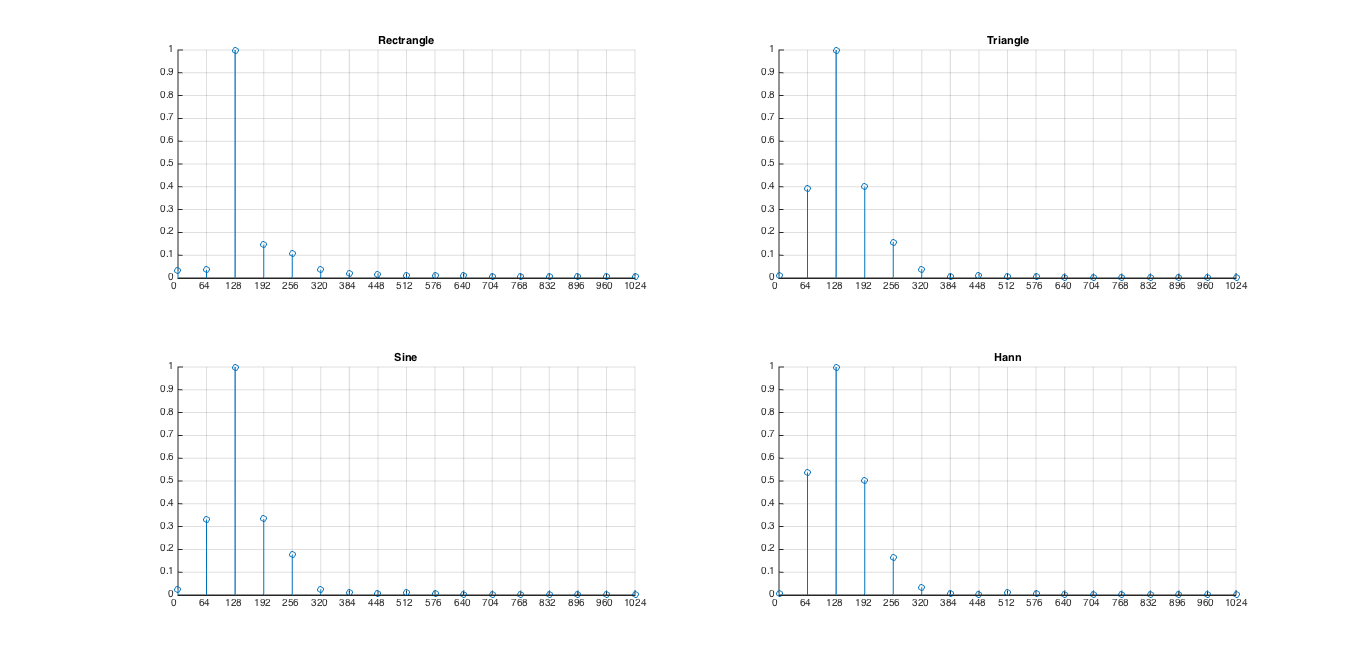
\includegraphics[width=1.1\textwidth]{WindowedSigDFT}}
    \label{WindowedSigDFT}
\end{figure}

\section{For each of the windowed signals in 3.1, zeropad each sequence to
length 2,048}
\begin{lstlisting}
function plot_windowed_signal(sig, win, Fs, plot_ind)
    sig = sig .* win;
    
    % Compute the DFT of the sine wave
    X = fft(sig, 2048);

    % Calculate normalized absolute magnitudes
    X = 20*log10(abs(X)/max(abs(X)));

    % Calculate DFT indexes
    n = 0:length(X)-1
    % Get DFT size
    N = length(n)
    % Calculate bin frequencies
    f = (n*Fs)/N

    % Create subplot
    subplot(2,2,plot_ind);
    hold on;
    % Plot DFT to the nyquist frequency
    plot(n(1:(end/2)+1), X(1:(end/2)+1))
    grid on;

    % Set axis ticks
    set(gca,'XTickMode','manual');
    set(gca,'XTick',0:64:N-1);
    set(gca,'XtickLabels', f(1:64:end));
    axis([0, 1024, -80, 5])
\end{lstlisting}

\begin{figure}[H]
    \caption{Normalized Magnitudes of 3 Tone Signal (DFT Size = 2048)}
    \makebox[\textwidth]{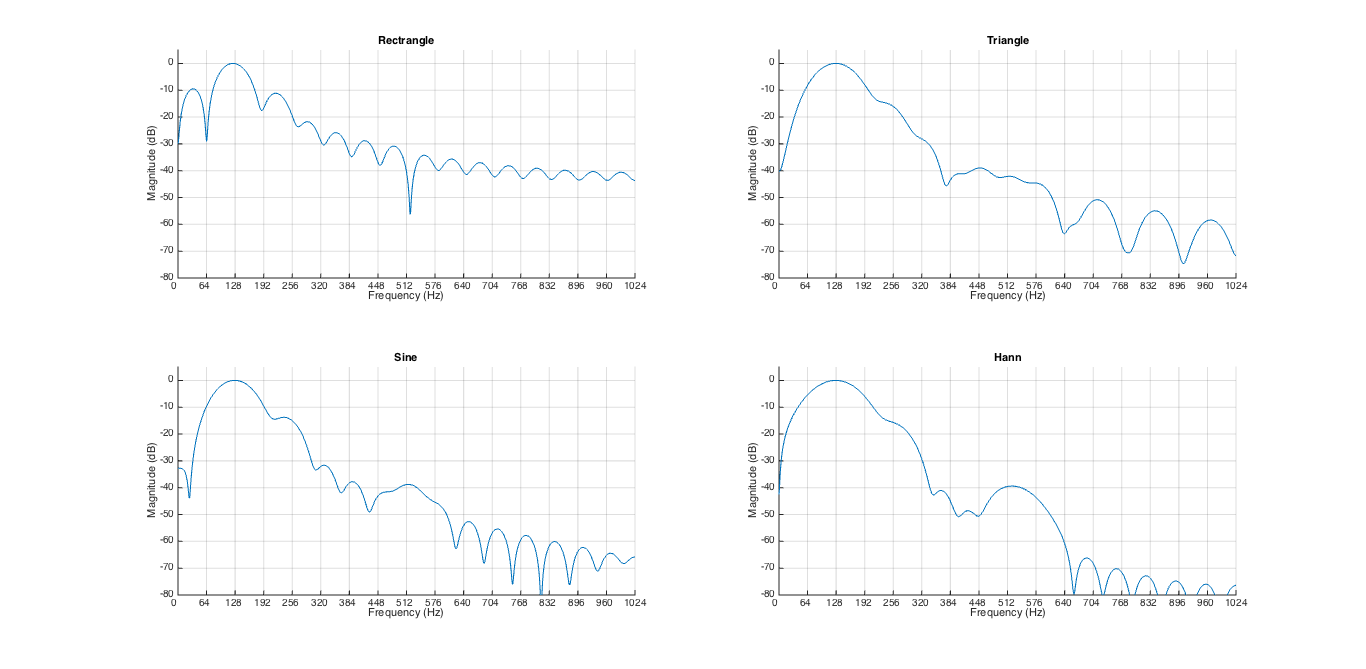
\includegraphics[width=1.1\textwidth]{WindowedSigDFT2048}}
    \label{WindowedSigDFT2048}
\end{figure}



\end{document}
